\documentclass{article}
\usepackage{nips15submit_e,times}
\usepackage{hyperref}
\usepackage{url}
\usepackage{amsmath}
\usepackage{amsfonts,amssymb}
\usepackage{graphicx}

\title{Weekly Report(July.30,2018-Aug.5,2018)}

\newcommand{\fix}{\marginpar{FIX}}
\newcommand{\new}{\marginpar{NEW}}

\begin{document}

\maketitle

\begin{abstract}
Sorry for my absence for two and a half weeks because of numerous assignments in school and social practice. In the last week, I have learned week5, week6 and week7 courses of \textbf{Machine Learning} and tried to run the code for \textbf{Object Detection}.
\end{abstract}

\section{Work done in this week}
\subsection{Neural Networks}
\subsubsection{Cost Function}
\begin{center}
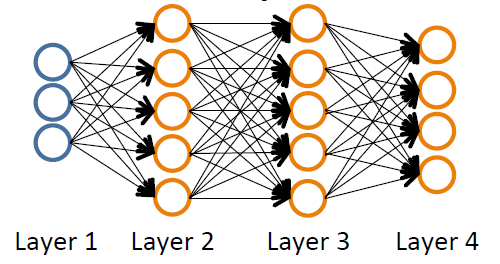
\includegraphics[scale=0.5]{pic.png}
\end{center}
Let's define a few variables that we will need:
\begin{itemize}
  \item L = total number of layers in the network
  \item s$_{l}$ = number of units (not counting bias unit) in layer 1
  \item K = number of output units/classes
\end{itemize}
Recall that the cost function for regularized logistic regression was:
\[J(\theta) = -\frac{1}{m}\sum^m_{i = 1}[y^{(i)}\log(h_{\theta}(x^{(i)}))+(1-y^{(i)})\log(1-h_{\theta}(x^{(i)}))]+\frac{\lambda}{2m}\sum^n_{j = 1}\theta_j^2\]
For neural networks, the cost function is going like this:
\[h_{\Theta}(x)\in\mathbb{R}^K \quad\quad (h_{\Theta}(x))_i\in i^{th} \text{output}\]
\[J(\Theta) = -\frac{1}{m}\sum_{i=1}^m\sum_{k=1}^K[y_k^(i)\log((h_{\Theta}(x^{(i)}))_k)+(1-y_k^{(i)})\log(1-(h_{\Theta}(x^{(i)}))_k)]+\frac{\lambda}{2m}\sum^{L-1}_{l=1}\sum^{s_l}_{i=1}\sum^{s_l+1}_{j=1}(\Theta_{j,i}^{(l)})^2\]
This is so confusing that I still couldn't fully understand it. How can I remember these complex cost functions and make good use of them?

\subsubsection{Backpropagation Algorithm}
To minimize our neural-network cost function, we use the Backpropagation algorithm:\\
We have the training set ${(x^{(1)},y^{(1)}),\ldots,(x^{(m)},y^{(m)})}$\\
Set $\Delta_{ij}^{(l)} = 0$ (for all $l,i,j$)\\
For $i = 1$ to $m$\\
$\qquad$Set $a^{(1)} = x^{(i)}$\\
$\qquad$Perform forward propagation to compute $a^{(l)}$ for $l = 2,3,\ldots,L$\\
$\qquad$Using $y^{(i)}$, compute $\delta^{(L)} = a^{(L)} - y^{(i)}$\\
$\qquad$Compute $\delta^{(L-1)},\delta^{(L-2)},\ldots,\delta^{(2)}$\\
$\qquad$$\Delta_{ij}^{(l)}:=\Delta_{ij}^{(l)}+a_j^{(l)}\delta_i^{(l+1)}$\\
$D_{ij}^{(1)}:=\frac{1}{m}\Delta_{ij}^{(l)}+\lambda\Theta_{ij}^{(l)}$ if $j\neq0$\\
$D_{ij}^{(1)}:=\frac{1}{m}\Delta_{ij}^{(l)}$ if $j=0$\\
$\frac{\partial}{\partial\Theta_{ij}^{(l)}}J(\Theta) = D_{ij}^{(l)}$\\
Here I have a problem with writing. How to add spaces correctly?
\begin{center}
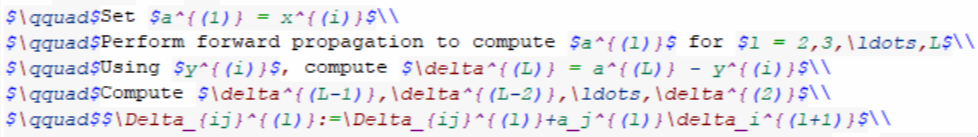
\includegraphics[scale=0.4]{2.png}
\end{center}
As I write in \LaTeX, I wanted to add some spaces in the beginning of my lines, but actually it didn't work.\\
To train a neural network, we can do as follows:
\begin{enumerate}
  \item Randomly initialize the weights
  \item Implement forward propagation to get $h_{\Theta}(x^{(i)})$ for any $x^{(i)}$
  \item Implement the cost function
  \item Implement backpropagation to compute partial derivatives
  \item Use gradient checking to confirm that your backpropagation works. Then disable gradient checking.
  \item Use gradient descent or a built-in optimization function to minimize the cost function with the weights in theta.
\end{enumerate}
\begin{center}
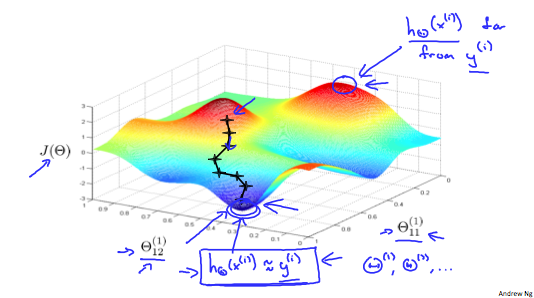
\includegraphics[scale=0.6]{3.png}
\end{center}
This image gives us an intuition of what is happening as we are implementing our neural network.

\subsection{Evaluating a Learning Algorithm}
Deciding what to try next is an essential part for us. Diagnostics can take time to implement, but doing so can be a very good use of our time.

\subsubsection{Evaluating our hypothesis}
\begin{itemize}
  \item Learn parameter $\theta$ from training data
  \item Compute test set error:
  \[J_{test}(\theta) = -\frac{1}{m_{test}}\sum_{i=1}^{m_{test}}y_{test}^{(i)}\log h_{\theta}(x_{test}^{(i)})+(1-y_{test}^{(i)})\log h_{\theta}(x_{test}^{(i)})\]
  \item Misclassification error(0/1 misclassification error):
\[err(h_{\Theta}(x),y) = \begin{cases}
1 & \text{if $h_{\Theta}(x) \geq 0.5$ and $y = 0$ or $h_{\Theta}(x) < 0.5$ and $y = 1$}\\
0 & \text{otherwise}
\end{cases}\]
\end{itemize}

\subsubsection{Model Selection}
Training error:
\[J_{train(\theta)} = \frac{1}{2m}\sum_{i=1}^m(h_{\theta}(x^{(i)}) - y^{(i)})^2\]
Cross Validation error:
\[J_{cv}(\theta) = \frac{1}{2m_{cv}}\sum_{i=1}^{m_{cv}}(h_{\theta}(x_{cv}^{(i)})-y_{cv}^{(i)})^2\]
Test error:
\[J_{test}(\theta) = \frac{1}{2m_{test}}\sum_{i=1}^{m_{test}}(x_{test}^{(i)})-y_{test}^{(i)})^2\]
In order to choose the model of your hypothesis, we can test each degree of polynomial and look at the error result. We can calculate three separate error values for the three different sets using the following method:
\begin{enumerate}
  \item Optimize the parameters in $\Theta$ using the training set for each polynomial degree.
  \item Find the polynomial degree d with the least error using the cross validation set.
  \item Estimate the generalization error using the test set with $J_{test}(\Theta^{(d)})$, (d = theta from polynomial with lower error);
\end{enumerate}

\subsubsection{Bias vs. Variance}
\textbf{High bias(underfitting):} both $J_{train}(\Theta)$ and $J_{CV}(\Theta)$ will be high. Also, $J_{CV}(\Theta) \approx J_{train}(\Theta)$.\\
\textbf{High variance(overfitting):} $J_{train}(\Theta)$ will be low and $J_{CV}(\Theta)$ will be low and $J_{CV}(\Theta)$ will be much greater than $J_{train}(\Theta)$.\\
The is summarized in the figure below:
\begin{center}
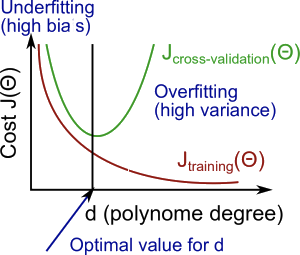
\includegraphics[scale=0.6]{4.png}
\end{center}

\subsubsection{Deciding What to Do Next Revisited}
We can do as follows:
\begin{itemize}
  \item \textbf{Getting more training examples:} Fixes high variance
  \item \textbf{Trying smaller sets of features:} Fixes high variance
  \item \textbf{Adding features:} Fixes high bias
  \item \textbf{Adding polynomial features:} Fixes high bias
  \item \textbf{Decreasing $\lambda$:} Fixes high bias
  \item \textbf{Increasing $\lambda$:} Fixes high variance.
\end{itemize}

\subsection{Support Vector Machines}
\subsubsection{SVM hypothesis}
\[\min\limits_{\theta}C\sum_{i=1}^m[y^{(i)}\cos t_1(\theta^Tx^{(i)}) + (1-y^{(i)})\cos t_0(\theta^Tx^{(i)})] + \frac{1}{2}\sum_{i=1}^n\theta_j^2\]
The C parameter is a positive value that controls the penalty for misclassified training examples.

\subsubsection{Large Margin Intuition}
\begin{center}
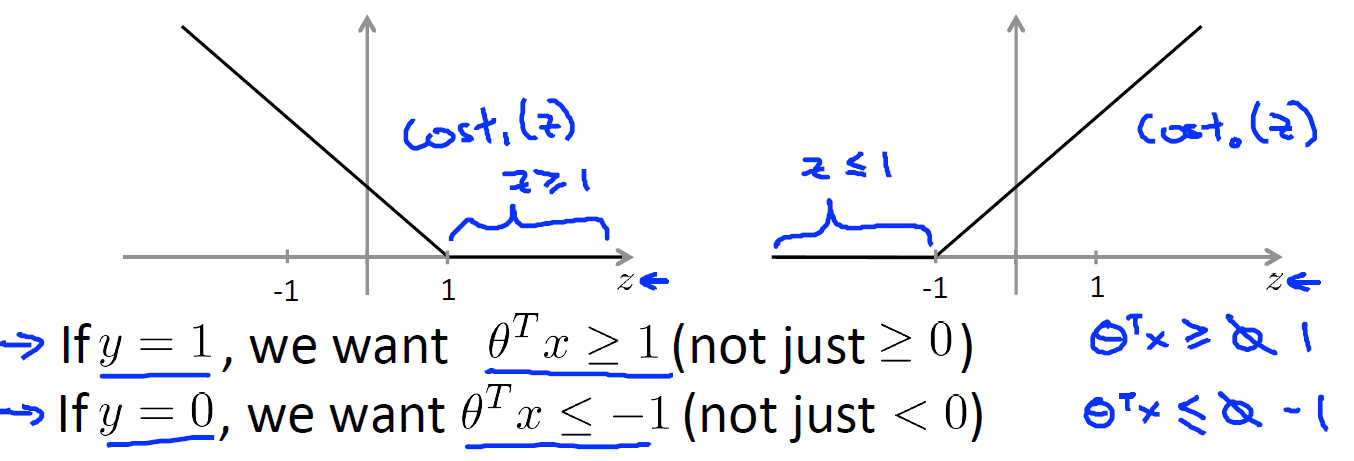
\includegraphics[scale=0.3]{6.png}
\end{center}
We can understand it intuitively from the image. Also, let's look at this image:
\begin{center}
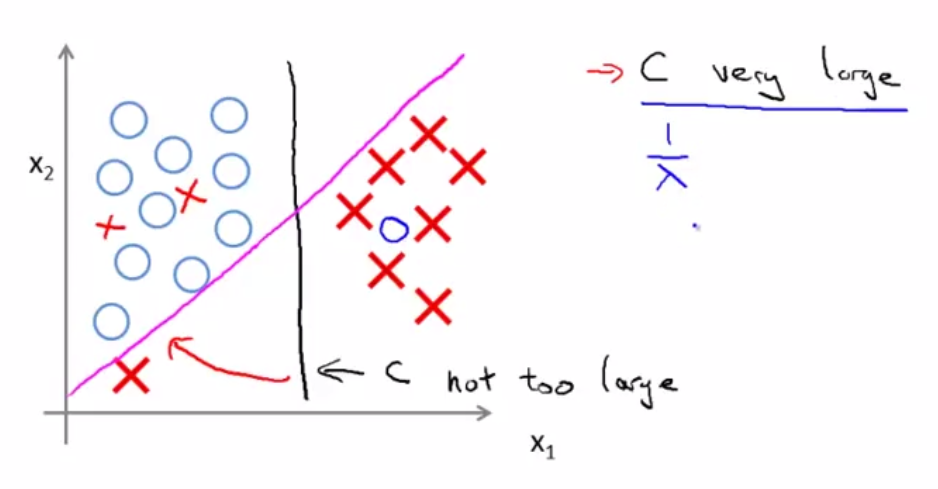
\includegraphics[scale=0.4]{5.png}
\end{center}
We can see that when C is not too large, we can get the black line. If C is too large, we get the pink line.

\subsubsection{Kernels}
When we're confronted with the case below, what should we do?
\begin{center}
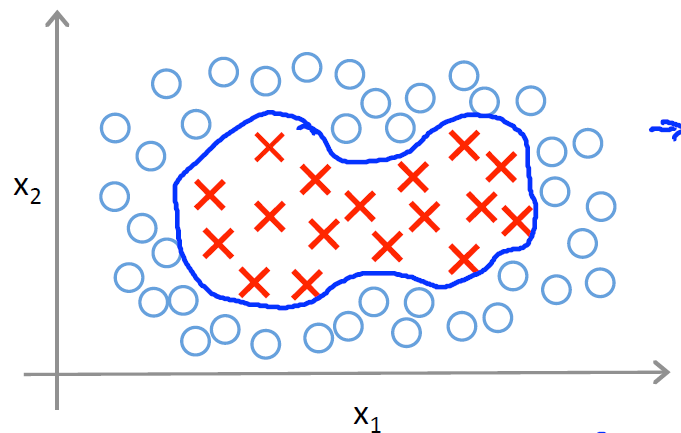
\includegraphics[scale=0.4]{7.png}
\end{center}
\textbf{Kernels and Similarity}
\[f_i = \text{similarity}(x,l^{(i)}) = \text{exp$(-\frac{\|x-l^{(i)}\|^2}{2\sigma^2})$}\]
Here is the example:
\begin{center}
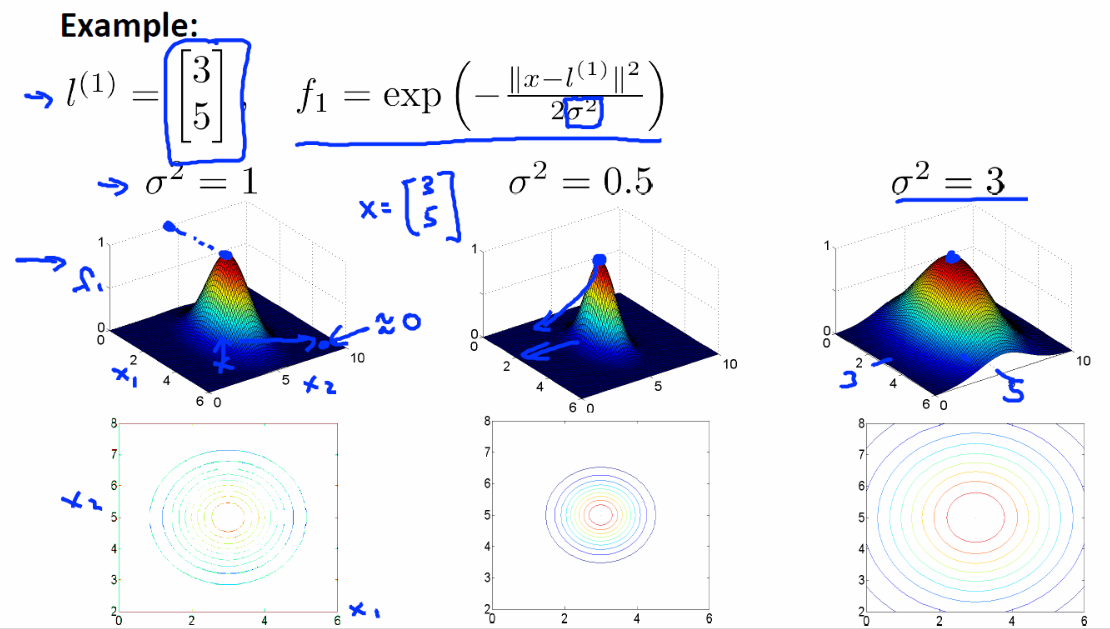
\includegraphics[scale=0.4]{8.png}
\end{center}
It is obvious that the $\sigma$ parameter determines the decreasing speed.
\textbf{SVM with Kernels}
Given $(x^{(1)},y^{(1)}),(x^{(2)},y^{(2)}),\ldots,(x^{m},y^{(m)})$\\
Choose $l^{(1)}=x^{(1)},l^{(2)}=x^{(2)},\ldots,l^{(m)}=x^{(m)}$\\
Given example x:
\[f_i = \text{similarity}(x,l^{(i)})\]
For training example $(x^{(i)},y^{(i)})$:
\[f_j^{(i)} = \text{similarity}(x^{(i)},l^{(j)})\]
And we can get that $C=\frac{1}{\lambda}$. Large C gets lower bias and high variance, And small C gets higher bias and low variance.

\subsection{Object Detection}
By running the \href{https://github.com/tensorflow/models/blob/master/research/object_detection/object_detection_tutorial.ipynb}{Object Detection Demo}, I got the rough outcome:
\begin{center}
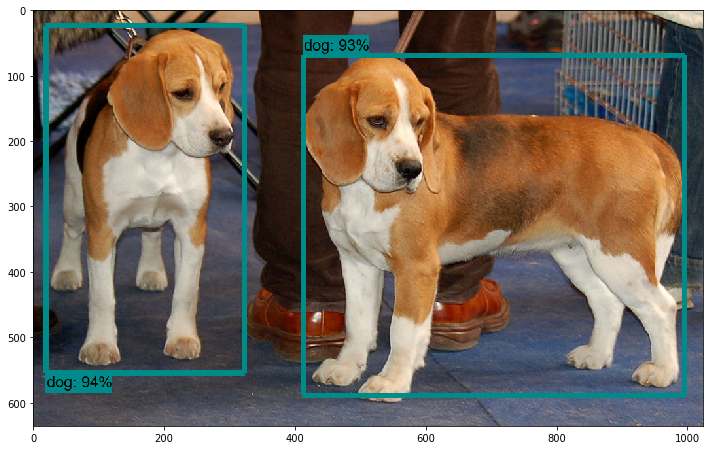
\includegraphics[scale=0.5]{index.png}
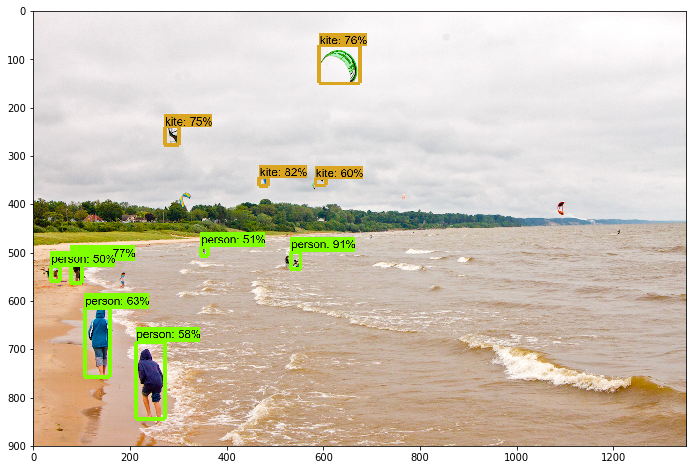
\includegraphics[scale=0.5]{index1.png}
\end{center}
The matching index is not very high, and I'm figuring how to make it better.

\section{Plans for Next Week}
\begin{enumerate}
  \item Learn the week8, week9, week10, week11 course of \textbf{Machine Learning}.
  \item Do more practices in Detection Networks.
\end{enumerate}

\end{document}
